% SPDX-License-Identifier: CC-BY-ND-4.0
\documentclass[
% handout,
aspectratio=169,
xcolor={usenames}
]{beamer}
% % To install handoutWithNotes from GitHub:
% % git clone https://github.com/gdiepen/latexbeamer-handoutWithNotes
% % cd latexbeamer-handoutWithNotes/
% % tlmgr install l3build
% % l3build install
% \usepackage{handoutWithNotes}
% \pgfpagesuselayout{4 on 1 with notes}[letterpaper, border shrink=5mm]
\graphicspath{ {img/} }
\setbeamertemplate{navigation symbols}{}
\setbeamertemplate{footline}[frame number]
\setbeamercolor{titlelike}{fg=white}
\setbeamercolor{author}{fg=white}
\setbeamercolor{institute}{fg=white}
\setbeamercolor{date}{fg=white}
\renewcommand{\footnoterule}{}
\usepackage{textpos}              % \textblock*
\addtobeamertemplate{frametitle}{%
  \begin{textblock*}{\paperwidth}(-28.3pt, 0pt)
    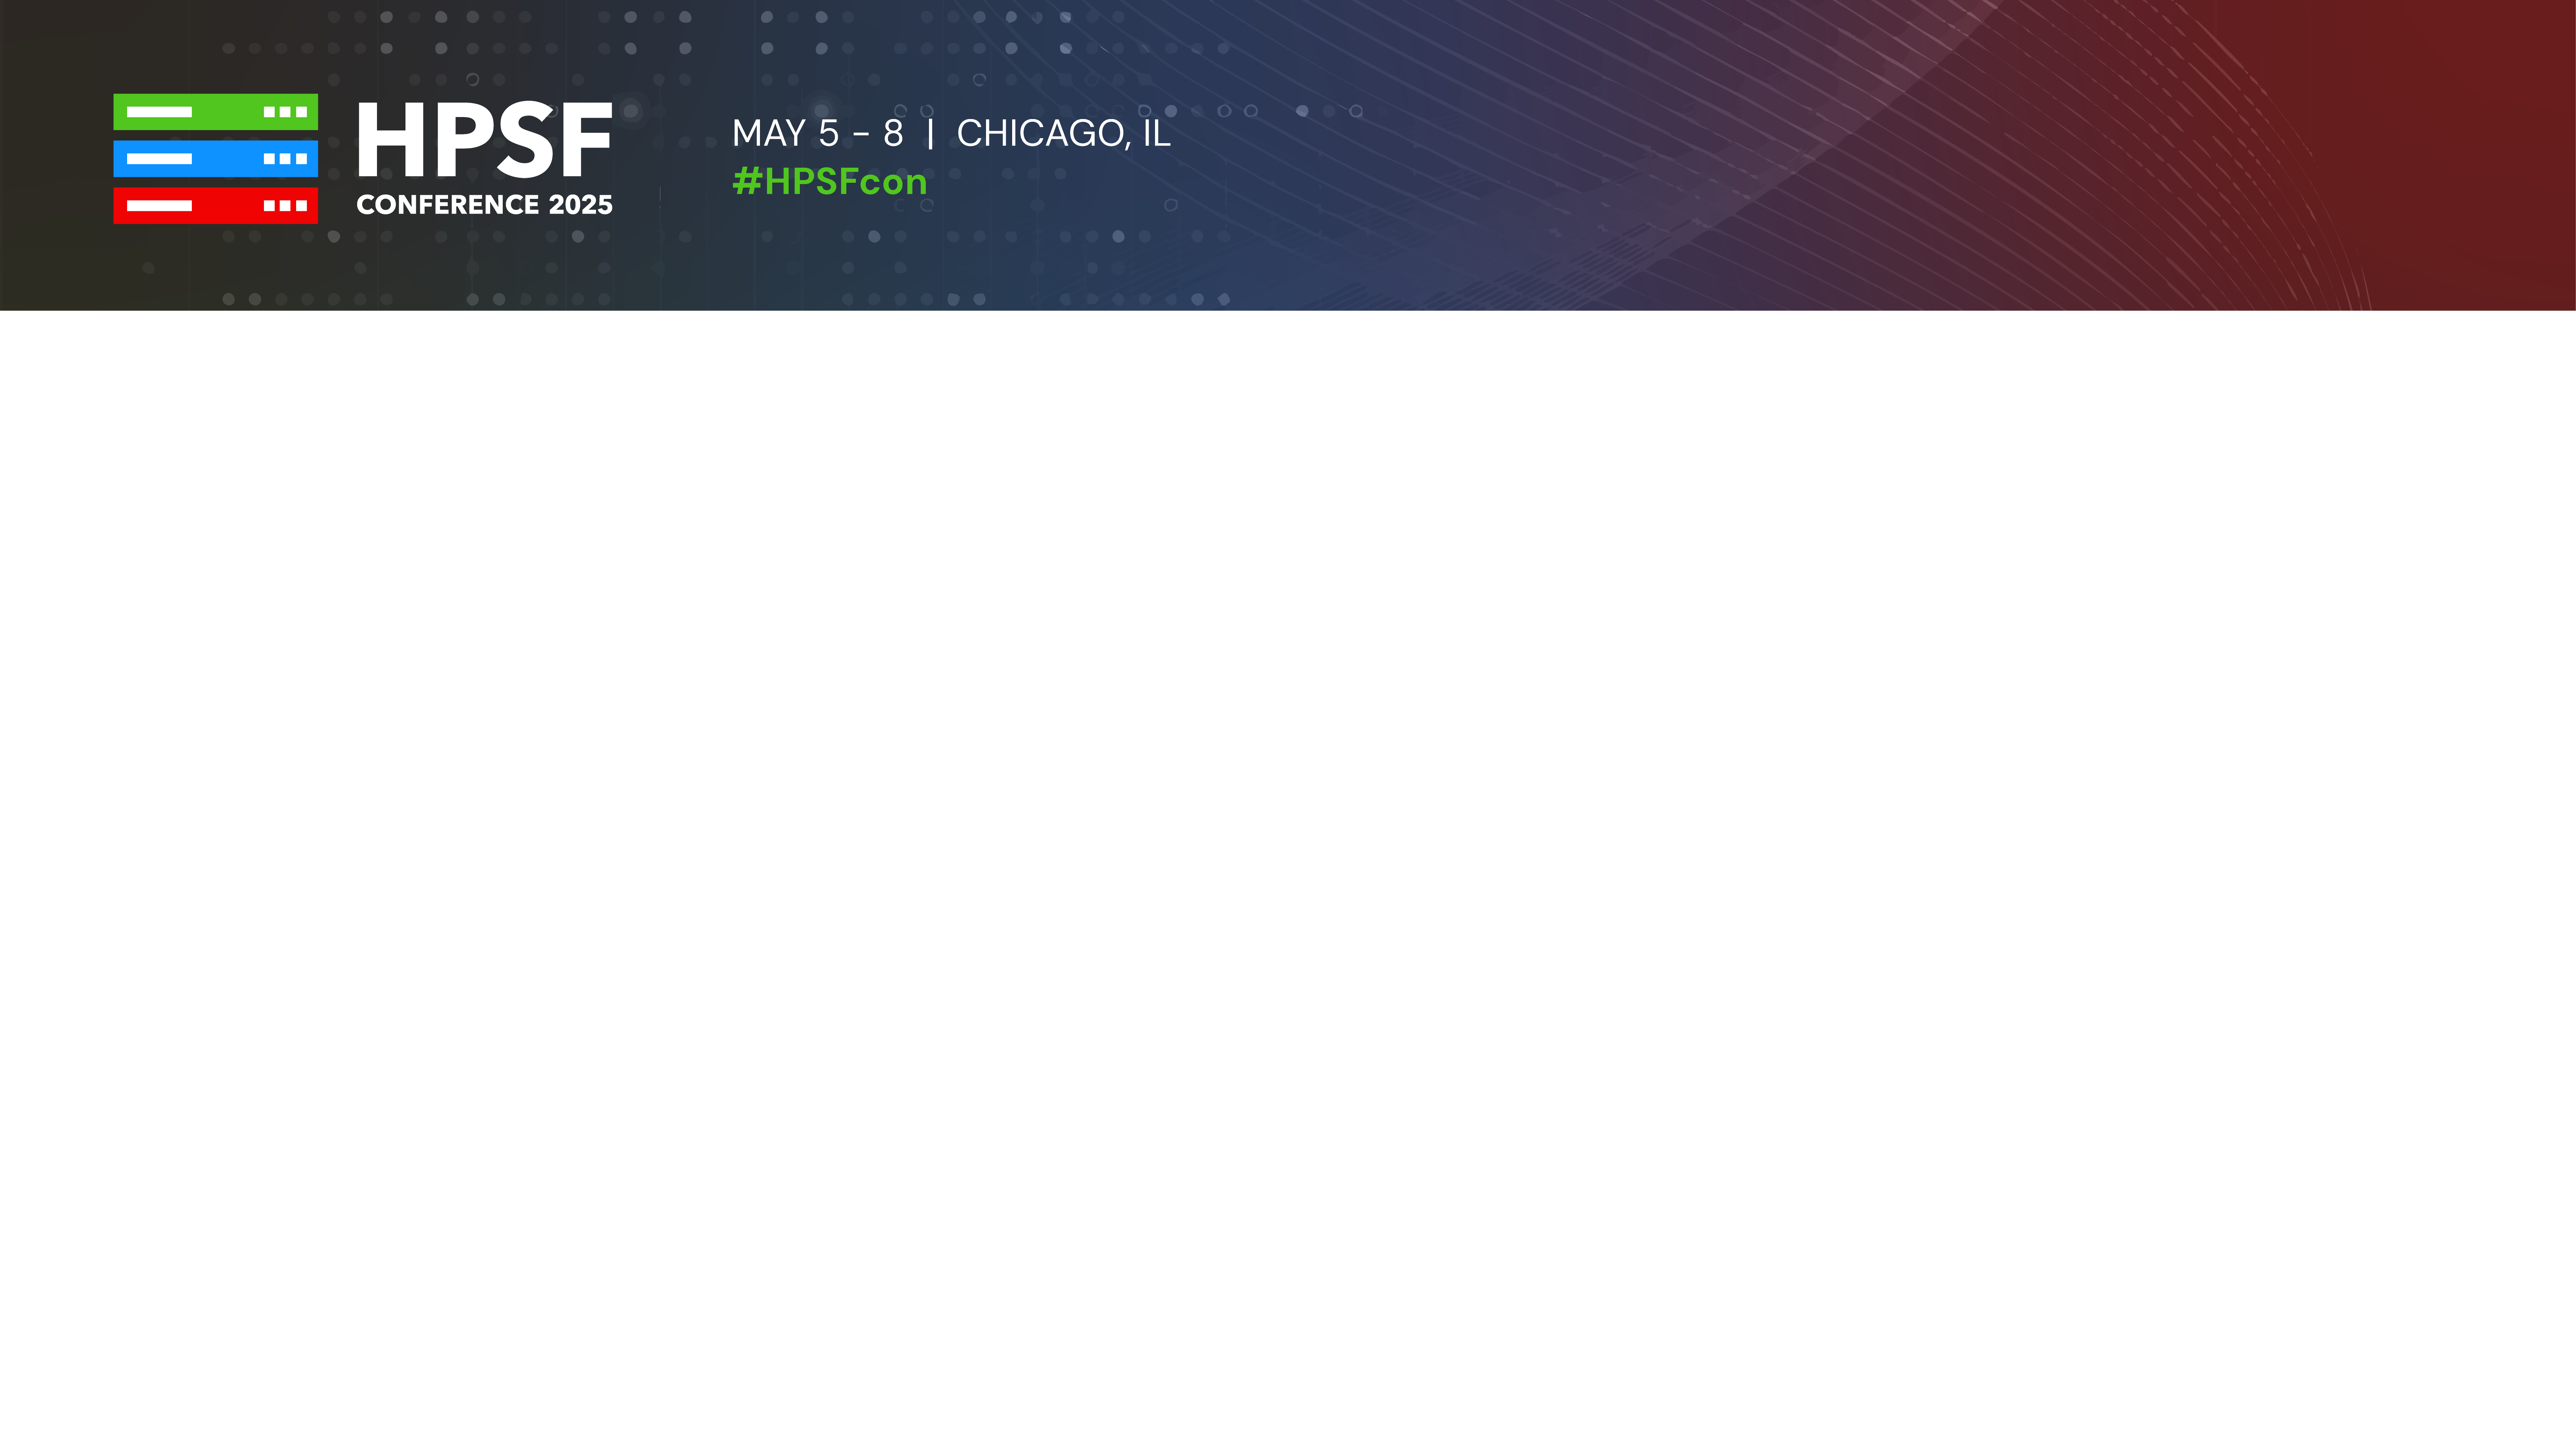
\includegraphics[width=\paperwidth]{im-hpsf-bg-slide.png}
  \end{textblock*}
  \vspace*{0.1cm}
}{
  % Adjust space between title and text per
  % https://latex.org/forum/viewtopic.php?p=92593#p92593
  \vspace*{0.4cm}
}

\usepackage[
backend=biber,
style=authoryear,
sorting=none
]{biblatex}
\addbibresource{\jobname.bib}

\usepackage{tikz}
\usetikzlibrary{calc}           % ($ ... $)
\usetikzlibrary{decorations.pathmorphing}    % zigzag
\usetikzlibrary{fit}            % fit
\usetikzlibrary{positioning}    % of
\usetikzlibrary{shapes.symbols} % signal
\tikzset{
  invisible/.style={opacity=0,text opacity=0},
  visible on/.style={alt=#1{}{invisible}},
  alt/.code args={<#1>#2#3}{%
    \alt<#1>{\pgfkeysalso{#2}}{\pgfkeysalso{#3}}
  },
}

\usepackage{soul}               % \ul

\usepackage{datetime2}          % \DTMnow

\title{Challenges mixing Spack-optimized %
  hardware accelerator libraries on %
  personal scientific computers}
\author{Pariksheet Nanda}
\institute{University of Pittsburgh\\%
  Chemical Engineering}
\date{May 8, 2025}

\begin{document}

\section{Title}

% Hide frame number on the title slide using noframenumbering,plain options per
% https://tex.stackexchange.com/a/317983
\begin{frame}[noframenumbering, plain]
  \begin{tikzpicture}[remember picture, overlay]
    \node at (current page.center) {%
      
\includegraphics[width=\paperwidth]{im-hpsf-bg-title.png}};
  \end{tikzpicture}
  \maketitle{}
\end{frame}

\section{Background}

\subsection{Background about myself}
\begin{frame}{\hspace{8cm}Background about myself}
  \begin{tikzpicture}[
    remember picture,
    overlay,
    timepoint/.style = {
      circle,
      fill = black,
      inner sep = 1pt
    },
    description/.style ={
      inner sep = 0pt,
      text width = 4.5cm
    }
    ]
    \coordinate (y07) at ($ (current page.west) +(+1,0) $);
    \coordinate (y24) at ($ (current page.east) +(-1,0) $);
    \coordinate (y16) at ($ (y07) !.4! (y24) $);
    \pgfmathparse{(2022 - 2016) / (2024 - 2016)}
    \coordinate (y22) at ($ (y16) !\pgfmathresult! (y24) $);
    \path [draw]
    (y07)
    node [timepoint] {}
    node [below] {2007}
    node [above, anchor = south] {
\includegraphics[scale=.1]{logo-gentoo.png}}
    node
    [description, below = .75 of y07, anchor = north west, xshift = -1cm] {
      \begin{itemize}[<+->]
      \item Low barrier from\\user $\to$ developer
      \item Use flags\\$\to$ spack variants
      \end{itemize}
    }
    decorate
    [decoration = {name = zigzag, pre length = 1cm, post length = 1cm}]
    { (y07) -- (y16) }
    (y16)
    node [timepoint] {}
    node [below] {2016}
    node [above, anchor = south] {\includegraphics<+->[scale=.3]{logo-sc16.png}}
    node [description, below = .75 of y16, anchor = north] {
      \begin{itemize}[<+->]
      \item<.-> HPC supervisor tells me about spack
      \item Installed 33 packages on university cluster
      \item Set spack as default on research lab server
      \end{itemize}
    }
    --
    (y22)
    node [timepoint] {}
    node [below] {2022}
    node [above, anchor = south] {%
      \includegraphics<+->[scale=0.45,clip,trim={8 8 10 5}]{im-gran.png}}
    node [description, below = .75 of y22, anchor = north, text width = 5cm,
    xshift = -1cm] {
      \begin{itemize}[<+->]
      \item<.-> Calibrate drug dosing for model of lung infection
      \item<.-> 2~week walltime
      \item<.-> Each sample 16~hrs
      \end{itemize}
    }
    --
    (y24)
    node [timepoint] {}
    node [below] {2024};
    \node at (y24) [above, text width = 1.8cm, visible on = {<+->}]
    {Wikipedia article: ``Spack (package $\phantom{(}$manager)''};
  \end{tikzpicture}
\end{frame}

\subsection{Motivation for this talk}
\begin{frame}{\hspace{8cm}Motivation for this talk}
  \begin{columns}[T]
    \begin{column}{.6\framewidth}
      \begin{itemize}[<+->]
      \item Laptops now come with neural processing units (NPUs)
        \begin{description}[<.->][2024]
        \item[2023] Intel Meteor Lake AI Boost
        \item[2023] AMD Ryzen XDNA
        \item[2024] Qualcomm Snapdragon X Hexagon
        \item[2024] M-series Apple Silicon Apple Intelligence
        \end{description}
      \item Bridging GPU / NPU scientific libraries %
        from Linux to Windows and macOS
      \item R (and python): NPU hardware optimization
      \end{itemize}
    \end{column}
    \begin{column}{.4\framewidth}
      \begin{tikzpicture}[%
        remember picture,
        overlay,
        every node/.style = {
          inner sep = 0pt,
          outer sep = 0pt
        }]
        \begin{scope}
          \coordinate (intel-center) at (1.5cm, -1cm);
          % Viewport.
          \clip ([xshift = -1.5cm, yshift = 1cm]intel-center)
          rectangle +(3cm, -2cm);
          \node (intel) at (intel-center) {%
            \includegraphics[height=2cm,clip,trim={0 135 30 130}]%
            {npu-intel.png}};
        \end{scope}
        \begin{scope}
          \coordinate [xshift = 3cm + 1pt] %
          (qualcomm-center) at (intel-center);
          % Viewport.
          \clip ([xshift = -1.5cm, yshift = -1cm]qualcomm-center)
          rectangle +(3cm, 2cm);
          \node (qualcomm) at (qualcomm-center) {%
            \includegraphics[height=2cm,clip,trim={0 110 0 130}]%
            {npu-qualcomm.jpg}};
        \end{scope}
        \begin{scope}
          \coordinate [yshift = -2cm -1pt] %
          (apple-center) at (qualcomm-center);
          % Viewport.
          \clip ([xshift = -1.5cm, yshift = -1cm]apple-center)
          rectangle +(3cm, 2cm);
          \node (apple) at (apple-center) {%
            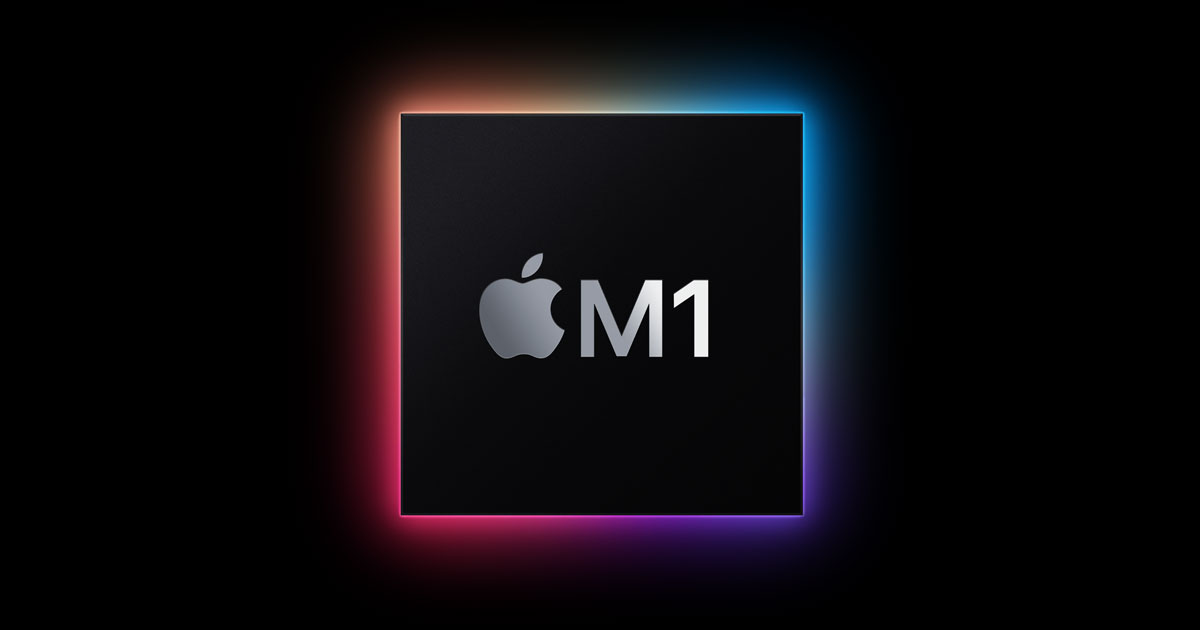
\includegraphics[height=2cm,clip,trim={0 55 0 55}]{npu-apple.jpg}};
        \end{scope}
        \begin{scope}
          \coordinate [yshift = -2cm -1pt] %
          (amd-center) at (intel-center);
          % Viewport.
          \clip ([xshift = -1.5cm, yshift = -1cm]amd-center)
          rectangle +(3cm, 2cm);
          \node (amd) at (amd-center) {%
            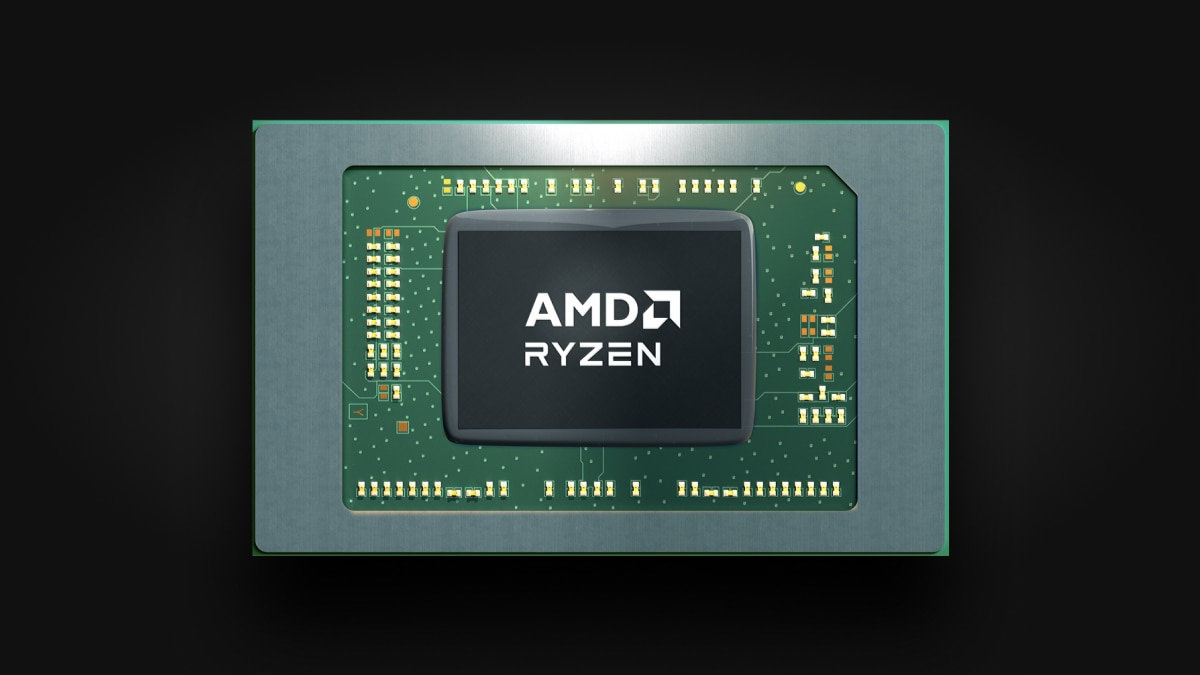
\includegraphics[height=2cm,clip,trim={0 170 0 170}]{npu-amd.jpg}};
        \end{scope}
      \end{tikzpicture}
    \end{column}
  \end{columns}
\end{frame}

\subsection{Foreign function interfaces (FFI) in R and python}
\begin{frame}{\hspace{8cm}Foreign function interfaces (FFI)\\%
    \hspace{8cm}in R and python}
  \begin{columns}[T]
    \begin{column}{.85\framewidth}
      \begin{itemize}[<+->]
      \item R
        \begin{itemize}
        \item<.-> Native extensions API (Fortran, C, C++) %
          easy to use and debug and %
          R seamlessly uses gcc / clang compiler
        \item Rcpp (C++) very widely used
        \end{itemize}
      \item Python
        \begin{itemize}
        \item<.-> Native C/C++ API extensions rarely used; too verbose
        \item Cython, cffi, SWIG, Numba
        \end{itemize}
      \item Mostly going to talk about R because of funding
      \end{itemize}
    \end{column}
    \begin{column}{.15\framewidth}
      \begin{tikzpicture}[%
        every node/.style = {
          inner sep = 0pt,
          outer sep = 0pt
        }
        ]
        \node (r)
        {
\includegraphics[width=.5\textwidth]{logo-r.png}};
        \node [anchor = west, xshift = 10pt, yshift = -2pt] (py) at (r.east)
        {
\includegraphics[width=.4\textwidth]{logo-python.png}};
        \node (lang) [%
        draw,
        fit = (r) (py),
        inner sep = 2pt,
        signal,
        signal pointer angle = 150,
        signal to = south] {};
        \path let \p1 = (lang.north west), \p2 = (lang.south east) in
        node (ffi) at (lang.south) [%
        anchor = north,
        yshift = -5pt,
        minimum width = \x2 - \x1,
        minimum height = \y1 - \y2,
        draw,
        signal,
        signal pointer angle = 150,
        signal from = north,
        signal to = south] {FFI};
        \path let \p1 = (lang.north west), \p2 = (lang.south east) in
        node (dots) at (ffi.south) [%
        anchor = north,
        yshift = -5pt,
        minimum width = \x2 - \x1,
        minimum height = \y1 - \y2,
        draw,
        signal,
        signal pointer angle = 150,
        signal from = north,
        signal to = south]
        {\ldots};
        \path let \p1 = (lang.north west), \p2 = (lang.south east) in
        node (npu) at (dots.south) [%
        anchor = north,
        yshift = -5pt,
        minimum width = \x2 - \x1,
        minimum height = \y1 - \y2,
        draw,
        signal,
        signal pointer angle = 150,
        signal from = north,
        signal to = nowhere] {NPU};
      \end{tikzpicture}
    \end{column}
  \end{columns}
\end{frame}

\subsection{GPU / NPU support in R has very little baggage}
\begin{frame}{\hspace{8cm}GPU / NPU support in R\\%
    \hspace{8cm}has very little ``baggage''}
  \begin{columns}[T]
    \begin{column}{.85\framewidth}
      \begin{itemize}[<+->]
      \item Current GPU R packages are {\color{alert}indirect}; %
        simply wrap around python / web interfaces %
        (tensorflow, keras3, ellmer, chattr)
      \item SYCL (compiler), Kokkos and RAJA (libraries) %
        are C++ vendor~neutral heterogeneous computing approaches
      \item But R is a GNU project; %
        hard to replace gcc with clang for SYCL support, %
        therefore need a library-approach like Kokkos
      \item<5-> Use case of Bioconductor R package system
      \end{itemize}
    \end{column}
    \begin{column}{.15\framewidth}
      \begin{tikzpicture}[%
        every node/.style = {
          inner sep = 0pt,
          outer sep = 0pt
        }
        ]
        \visible<4->{
          \node (kokkos) [%
          draw,
          inner sep = 2pt,
          signal,
          signal pointer angle = 150,
          signal from = north,
          signal to = south]
          {
\includegraphics[width=\textwidth]{logo-kokkos.png}};
        }
        \path let \p1 = (kokkos.north west), \p2 = (kokkos.south east) in
        node (ffi) at (kokkos.north) [%
        anchor = south,
        yshift = 5pt,
        minimum width = \x2 - \x1,
        minimum height = \y1 - \y2,
        draw,
        signal,
        signal pointer angle = 150,
        signal from = north,
        signal to = south] {FFI};
        \path let \p1 = (kokkos.north west), \p2 = (kokkos.south east) in
        node (r) at (ffi.north) [%
        anchor = south,
        yshift = 5pt,
        minimum width = \x2 - \x1,
        minimum height = \y1 - \y2,
        draw,
        inner sep = 2pt,
        signal,
        signal pointer angle = 150,
        signal from = nowhere,
        signal to = south]
        {
\includegraphics[width=.5\textwidth]{logo-r.png}};
        \visible<-3|handout:0>{
          \path let \p1 = (kokkos.north west), \p2 = (kokkos.south east) in
          node (dots) at (kokkos) [%
          minimum width = \x2 - \x1,
          minimum height = \y1 - \y2 - 5pt,
          draw,
          signal,
          signal pointer angle = 150,
          signal from = north,
          signal to = south]
          {\ldots};
        }
        \path let \p1 = (kokkos.north west), \p2 = (kokkos.south east) in
        node (npu) at (kokkos.south) [%
        anchor = north,
        yshift = -5pt,
        minimum width = \x2 - \x1,
        minimum height = \y1 - \y2,
        draw,
        signal,
        signal pointer angle = 150,
        signal from = north,
        signal to = nowhere] {NPU};

        \visible<1|handout:0>{
          \draw [color = alert, line width = 2]
          ($ (ffi.north west) + (-5pt,+5pt) $) --
          ($ (npu.south east) + (+5pt,-5pt) $)
          ($ (ffi.north east) + (+5pt,+5pt) $) --
          ($ (npu.south west) + (-5pt,-5pt) $);
        }
      \end{tikzpicture}
    \end{column}
  \end{columns}
\end{frame}

\subsection{Bioconductor R packages for biological sciences}
\begin{frame}{\hspace{8cm}Bioconductor R packages\\%
    \hspace{8cm}for biological sciences}
  \begin{columns}[T]
    \begin{column}{.85\framewidth}
      \begin{itemize}[<+->]
      \item Since 2001 by R co-creator Robert Gentleman
        \begin{itemize}[<.->]
        \item $\ge 2000$ packages, %
          $\approx 150k$ unique IP address downloads\footnotemark[1]
        \item Impact of 5000--6000 yearly citations since 2019\footnotemark[1]
        \end{itemize}
      \item CI rebuilds all packages every 48 hours:
        \begin{itemize}[<.->]
        \item Windows Server 2022 (x86\_64)
        \item macOS 12, 13 (x86\_64, aarch64)
        \item Ubuntu Linux 24 (x86\_64, aarch64)
        \end{itemize}
      \item Bioconductor released their first GPU package, RbowtieCuda, %
        last month (April) --- not vendor neutral
      \end{itemize}
    \end{column}
    \begin{column}{.15\framewidth}
      \begin{tikzpicture}
        \node (bioc)
        {
\includegraphics[width=\textwidth]{logo-bioconductor.png}};
        \node (r) at (bioc.south) [anchor = north, yshift = -20pt]
        {
\includegraphics[width=\textwidth]{logo-r.png}};
        \draw [-stealth, line width = 2pt] (bioc) -- (r);
      \end{tikzpicture}
    \end{column}
  \end{columns}
  \footnotetext[1]{%
    Bioconductor Annual Report 2024: \url{https://bioconductor.org/about/annual-reports/}}
\end{frame}

\section{Proposal}

\subsection{Proposed R stack for Kokkos NPU support}
\begin{frame}{\hspace{8cm}Proposed R stack\\%
    \hspace{8cm}for Kokkos NPU support}
  \begin{columns}[T]
    \begin{column}{.85\framewidth}
      \begin{itemize}[<+->]
      \item Bioconductor S4 classes %
        allow strict package interoperability; %
        versioning scheme similar to OS release process
      \item Provide R API that encapsulates Kokkos C++ stack using 2~packages
        \begin{enumerate}
        \item<.-> S4 \ul{class} interface
          \begin{itemize}[<.->]
          \item DelayedArray, DelayedTensor S4 classes
          \item Wrap \#bio-kokkos algorithms / kernels
          \end{itemize}
        \item Expose Kokkos backend \ul{runner} for BiocParallel
          \begin{itemize}
          \item<.-> Existing backends: %
            single CPU, %
            multicore, %
            socket cluster, %
            Redis cluster, %
            MPI cluster, %
            Batchtools (SLURM, etc.)
          \item Possible future feature of combining backends %
            (MPI with Multicore, MPI with BiocKokkos, etc.)
          \end{itemize}
        \end{enumerate}
      \end{itemize}
    \end{column}
    \begin{column}{.15\framewidth}
      \begin{tikzpicture}[%
        every node/.style = {
          inner sep = 0pt,
          outer sep = 0pt
        }
        ]
        \node (kokkos) [%
        draw,
        inner sep = 2pt,
        signal,
        signal pointer angle = 150,
        signal from = north,
        signal to = south]
        {
\includegraphics[width=\textwidth]{logo-kokkos.png}};
        \path let \p1 = (kokkos.north west), \p2 = (kokkos.south east) in
        node (ffi) at (kokkos.north) [%
        anchor = south,
        yshift = 5pt,
        minimum width = \x2 - \x1,
        minimum height = \y1 - \y2,
        draw,
        signal,
        signal pointer angle = 150,
        signal from = north,
        signal to = south] {FFI};
        \visible<2->{
          \path let \p1 = (kokkos.north west), \p2 = (kokkos.south east) in
          node (class) at (ffi.north) [%
          anchor = south,
          yshift = 5pt,
          minimum width = \x2 - \x1,
          draw,
          inner sep = 2pt,
          signal,
          signal pointer angle = 150,
          signal from = north,
          signal to = south]
          {BiocKokkos};
        }
        \visible<3->{
          \path let \p1 = (class.north west), \p2 = (class.south east) in
          node (bp) at (class.north) [%
          anchor = south,
          yshift = 5pt,
          minimum width = \x2 - \x1,
          draw,
          inner sep = 2pt,
          signal,
          signal pointer angle = 150,
          signal from = nowhere,
          signal to = south]
          {BiocParallel};
        }
        \visible<-1|handout:0>{
          \path let \p1 = ($ (bp.north west) + (0, 5pt) $),
          \p2 = (class.south east) in
          node (r) at (ffi.north) [%
          anchor = south,
          yshift = 5pt,
          minimum width = \x2 - \x1,
          minimum height = \y1 - \y2,
          draw,
          inner sep = 2pt,
          signal,
          signal pointer angle = 150,
          signal from = nowhere,
          signal to = south]
          {
\includegraphics[width=.5\textwidth]{logo-r.png}};
        }
        \path let \p1 = (kokkos.north west), \p2 = (kokkos.south east) in
        node (npu) at (kokkos.south) [%
        anchor = north,
        yshift = -5pt,
        minimum width = \x2 - \x1,
        minimum height = \y1 - \y2,
        draw,
        signal,
        signal pointer angle = 150,
        signal from = north,
        signal to = nowhere] {NPU};
      \end{tikzpicture}
    \end{column}
  \end{columns}
\end{frame}

\subsection{Proposed OS roadmap  and vendor interest}
\begin{frame}{\hspace{8cm}Proposed OS roadmap\\%
    \hspace{8cm}and vendor interest}
  \begin{columns}[T]
    \begin{column}{.81\framewidth}
      \begin{itemize}[<+->]
      \item Spack kokkos GPU development environment %
        on remaining operating systems:
        \begin{itemize}
        \item<.-> Windows 11 LXC container by Canonical\footnotemark[1] %
          [Bioconductor production uses Azure builder]
        \item Apple license %
          limits running macOS on Apple hardware (Mac mini) %
          [Bioconductor production uses MacStadium.com]\footnotemark[2]
        \end{itemize}
      \item Ideally, vendors would help support Kokkos (e.g. via SYCL):
        \begin{itemize}
        \item<.-> nVidia points to their Clara Parabricks containers, %
          but needs 16GB GPU RAM, not open source(?)
        \item Apple receptive, %
          but need to build the business case %
          for systems engineering software support of clang SYCL
        \end{itemize}
      \end{itemize}
    \end{column}
    \begin{column}{.19\framewidth}
      \begin{tikzpicture}
        \node {
\includegraphics[width=\textwidth]{logo-lxc.png}};
      \end{tikzpicture}
    \end{column}
  \end{columns}
  \footnotetext[1]<1->{Not sure about GPU support in LXC container}
  \footnotetext[2]<2->{What sandboxes you are using for macOS %
    that exposes the GPU?}
\end{frame}

\section{Wrap up}

\subsection{Landscape of software alternatives}
\begin{frame}{\hspace{8cm}Landscape of software alternatives}
  \begin{columns}[T]
    \begin{column}{.75\framewidth}
      \begin{itemize}[<+->]
      \item Only competitor seems to be %
        is bioc2u (based on r2u) %
        of Bioconductor packages on Ubuntu
        \begin{itemize}
        \item<.-> Running %
          \texttt{install.packages(...)} %
          uses a repository of
          \ul{precompiled OS packages} instead of Bioconductor sources
        \item Uses \texttt{bspm R} package (Bridge to System Package Manager)
          root privilege escalation via inter-process communication (IPC)
        \item Demonstrates need for a project like spack
          \begin{itemize}
          \item<.-> Keep package source and link to externals with spack
          \item Support distros besides Ubuntu
          \item Could automatically parse configure errors %
            to install the relevant spack packages %
            (like TinyTex does for LaTeX)
          \end{itemize}
        \end{itemize}
      \end{itemize}
    \end{column}
    \begin{column}{.25\framewidth}
      \begin{tikzpicture}
        \node (bioc)
        {
\includegraphics[width=.3\textwidth]{logo-bioconductor.png}};
        \node [anchor = north, yshift = -20pt] (r) at (bioc.south)
        {
\includegraphics[width=.3\textwidth]{logo-r.png}};
        \node [anchor = east] (ubuntu) at (bioc.west)
        {
\includegraphics[width=.3\textwidth]{logo-ubuntu.png}};
        \visible<4->{
          \node [anchor = west] (spack) at (bioc.east) 
          {
\includegraphics[width=.3\textwidth]{logo-spack.pdf}};
          \draw [-stealth, line width = 2pt] (spack) -- (r);
        }
        \draw [-stealth, line width = 2pt] (bioc) -- (r);
        \visible<-3>{
          \draw [-stealth, line width = 2pt] (ubuntu) -- (r);
          \coordinate (mid) at ($ (bioc) !.5! (r) $);
          \draw [color = alert, line width = 2pt]
          (mid) +(-5pt,+5pt) -- +(+5pt,-5pt)
          (mid) +(+5pt,+5pt) -- +(-5pt,-5pt);
          \draw [-stealth, line width = 2pt]
          (bioc) to [out = 120, in = 60, looseness = 2] (ubuntu);
        }
      \end{tikzpicture}
    \end{column}
  \end{columns}
\end{frame}

\subsection{4 projects we can work on independently}
\begin{frame}{\hspace{8cm}4 projects we can work on\\%
    \hspace{8cm}independently}
  \begin{enumerate}[<+->]
  \item Spack \texttt{bspm} backend to seamlessly install spack packages from R
  \item Spack concretizer ``release'' versioning constraints
    \begin{itemize}[<.->]
    \item e.g. Operating systems, Bioconductor
    \end{itemize}
  \item Kokkos OS support on %
    Windows $\ge 10$\footnotemark[1]
    (Intel Meteor Lake, AMD Ryzen XDNA, Qualcomm Snapdragon X) and %
    macOS $\ge 13.5$\footnotemark[2]
    (Apple silicon)
  \item Bioconductor R packages\footnotemark[3]:
    \begin{description}[S4 R class]
    \item[S4 R class]<.-> %
      interface with DelayedTensor/Array R packages, Kokkos C++
    \item[Runner] BiocParallel Kokkos backend
    \end{description}
  \end{enumerate}
  \footnotetext[1]<3->{Support for Microsoft Copilot}
  \footnotetext[2]<3->{Support for Apple Metal Machine Learning Explore (MLX)}
  \footnotetext[3]<4->{Will gauge interest at the Bioconductor conference this June}
\end{frame}

\section{Thank you}

\begin{frame}[noframenumbering, plain]
  \begin{tikzpicture}[remember picture, overlay]
    \node at (current page.center) {%
      
\includegraphics[width=\paperwidth]{im-hpsf-bg-title.png}};
  \end{tikzpicture}
  \color{white}
  \begin{center}
    \LARGE Thank you!
  \end{center}
  \let\thefootnote\relax\footnotetext{\hfill{}\color{white}\DTMnow{}}
\end{frame}

\end{document}
